%%% LaTeX Template
%%% This template can be used for both articles and reports.
%%%
%%% Copyright: http://www.howtotex.com/
%%% Date: February 2011

%%% Preamble
\documentclass[paper=a4, fontsize=12pt]{scrartcl}	% Article class of KOMA-script with 11pt font and a4 format
\usepackage[margin=0.7in]{geometry}
\usepackage[english]{babel}															% English language/hyphenation
\usepackage[protrusion=true,expansion=true]{microtype}				% Better typography
\usepackage{amsmath,amsfonts,amsthm}										% Math packages
%\usepackage{color,transparent}													% If you use color and/or transparency
\usepackage[hang, small,labelfont=bf,up,textfont=it,up]{caption}	% Custom captions under/above floats
\usepackage{epstopdf}																	% Converts .eps to .pdf
\usepackage{subfig}																		% Subfigures
\usepackage{booktabs}																	% Nicer tables
\usepackage[pdftex]{graphicx}
\usepackage{listings}
\usepackage{lscape}
\usepackage{longtable}
\usepackage{dcolumn}
\usepackage{caption}
\usepackage{subfig}

%%% Advanced verbatim environment
\usepackage{verbatim}
\usepackage{fancyvrb}
\DefineShortVerb{\|}								% delimiter to display inline verbatim text


%%% Custom sectioning (sectsty package)
\usepackage{sectsty}								% Custom sectioning (see below)
\allsectionsfont{%									% Change font of al section commands
	\usefont{OT1}{bch}{b}{n}%					% bch-b-n: CharterBT-Bold font
%	\hspace{15pt}%									% Uncomment for indentation
	}

\sectionfont{%										% Change font of \section command
	\usefont{OT1}{bch}{b}{n}%					% bch-b-n: CharterBT-Bold font
	\sectionrule{0pt}{0pt}{-5pt}{0.8pt}%	% Horizontal rule below section
	}


%%% Custom headers/footers (fancyhdr package)
\usepackage{fancyhdr}
\pagestyle{fancyplain}
\fancyhead{}														% No page header
\fancyfoot[C]{\thepage}										% Pagenumbering at center of footer
\renewcommand{\headrulewidth}{0pt}				% Remove header underlines
\renewcommand{\footrulewidth}{0pt}				% Remove footer underlines
\setlength{\headheight}{13.6pt}

%%% Equation and float numbering
\numberwithin{equation}{section}															% Equationnumbering: section.eq#
\numberwithin{figure}{section}																% Figurenumbering: section.fig#
\numberwithin{table}{section}

\usepackage[parfill]{parskip}
\usepackage{float}
\usepackage{hyperref}
\usepackage[numbers]{natbib}															% Tablenumbering: section.tab#

% use sans-serif font
\renewcommand{\familydefault}{\sfdefault}

%%% Title
\title{
	\vspace{-0.5in} 	\usefont{OT1}{bch}{b}{n}
        SEM2220: Have smartphones revolutionized the way we shop? \
}

% Authors
\author{
	\usefont{OT1}{bch}{m}{n} User ID: 110036072
	\\ \usefont{OT1}{bch}{m}{n} Aberystwyth University 
%%	\\   \texttt{slj11@aber.ac.uk}
}

\date{\today}

\begin{document}

\maketitle

\section{Introduction}
The advent of smartphones in the early 21$^{st}$ century has had a dramatic social impact on everyday life. This essay asks the question ``Have smartphones revolutionized the way we shop?''. Based on the evidence presented in this report I would be inclined to argue that they have and will continue to do so.

The number of smartphone users worldwide continues to increase worldwide with the total number of smartphone users expected to surpass the 2 billion mark by the end of 2017 \cite{emarketer2016smartphone}. As the number of smartphone users is forecasted to increase, so is the number of mobile internet users \cite{statista2016mobile}. In the UK alone, Ofcom reports that 61\% of people used their mobile to access the internet last year \cite{ofcom2016facts}. Furthermore, the threshold where more users access digital content in the US via a mobile connection rather than by desktop has already been surpassed \cite{comscore2014us}. Based on evidence such as this it cannot be denied that the mobile platform is increasingly becoming a fundamental part of peoples lives. The uptake in users of the mobile web suggests that people are becoming more connected anywhere they are. This at least sets the foundation for significant number of people to be ready to utilise mobile commerce.

\begin{figure}[H]
\centering
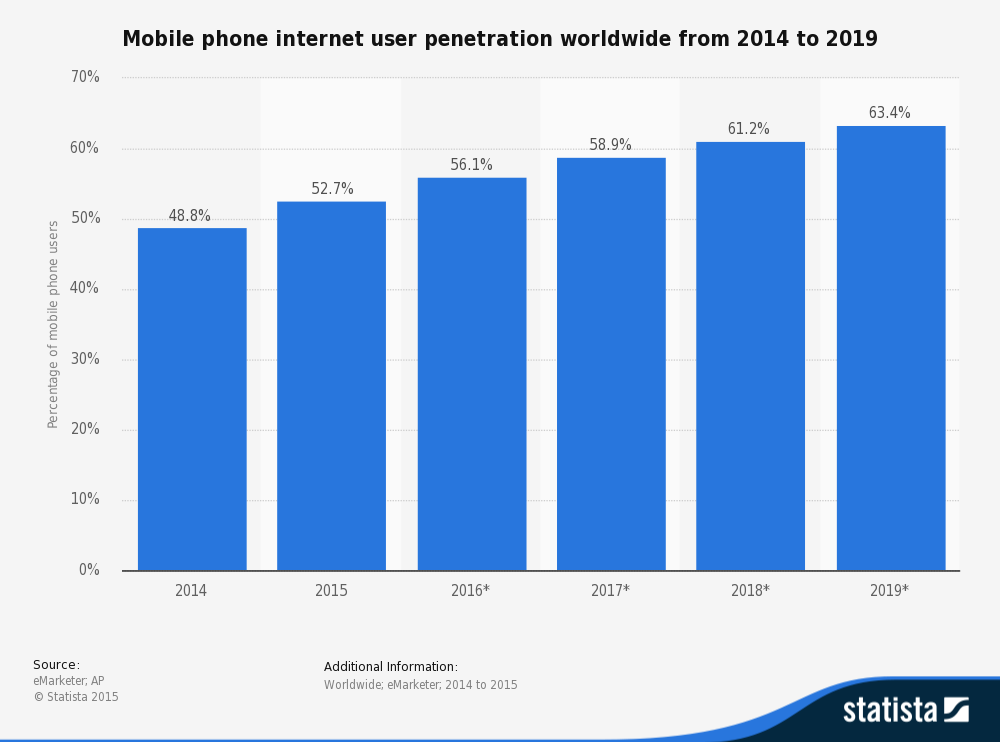
\includegraphics[width=0.5\textwidth]{img/statistic-mobile-phone-internet-user-penetration-worldwide-2014-2019.png}
\caption{Mobile phone internet user statistics and forecast from 2014-2019. Years marked with an asterisk are estimates. Image source: Statista \cite{statista2016mobile}.}
\label{fig:}
\end{figure}

\section{Mobile Commerce Technology}

The number of ways in which consumers can perform transactions through their mobile devices has been increasing since the introduction of modern smartphones in the early years of the millennium. In the most basic form, having mobile access to the internet is an enabler for commerce. Even without custom mobile apps and the mobile web the mere ability for users to access websites wherever they are facilitates a new avenue for reaching the consumer. 

I would argue that this was the first boost provided by the mobile industry to commerce. The advent of the Internet had already revolutionised the way people shop. The effect that this has had on high street stores and how big online retailers (eBay, Amazon etc.) have come to dominate the online marketplace \cite{}. The introduction of the mobile web has led to consumers being able to purchase goods from anywhere with an internet connection, something which is now classed as a human right \cite{}. 

The availability of this content has led to a change in the way consumers evaluate cost and deals. Mobile internet access allows users to access price information in real time. This has been an essential boost for some companies such as eBay which rely on user's accessing real time prices. But in a wider context user can be much more savvy in how they shop. It is now trivial to check if a deal offered in a store can be bettered by a competitor, without leaving store. In fact some companies now offer to beat their online competitors \cite{}.

As the uptake of mobile phones became apparent, mobile app marketplaces added new opportunities for getting your products to consumers. Many large businesses offer native mobile applications for there online store (e.g. Amazon, eBay). But this concept has been taken further. Some companies, for example GBK \cite{}, offer apps which will offer the user ``points'' collected by purchases which can lead to discounts, replacing the traditional paper discount card. This also provides the company with a way to further market there product to the user.

Microtransactions, transactions involving very small sums of money exchanged over the internet have come to dominate the revenue stream from app marketplaces \cite{venture2014report}, particularly amongst the games market \cite{mashable2015micro}. I would argue that this has potentially led to an increase in expenditure with mobile marketplaces. When app marketplaces where first most were separated into free and paid applications. Now with microtransactions often baked into apps many are often free to download and use with limited functionality, but cost to upgrade or add additional features.

The world is now seeing the rise of mobile point-of-sale (mPOS) technology (such as the services offered by PayPal, Square, Intuit, VeriFone etc.) for business owners and online wallets (Apple Pay, Google Wallet, Amazon Payments, etc.) for customers which brings more transaction options into the world, especially when in conjunction with near field communication (NFC) technology. Adoption of these technologies beyond the boarders of the U.S have yet to be fully realised. There is also increasingly the use of paying for goods and services by scanning barcodes of QR codes at the POS or for registration for later payment. 

Time is yet to tell what the next major payment system will be or whether full uptake of mobile payment systems will ever be fully realised. Could such technology lead to the rise of cashless societies? Given that the uptake of credit/debit card and chip \& pin services have failed to kill of physical cash as a form payment this seems unlikely, at least in the near future. I would perhaps argue that the speed of contactless NFC payment and the ease of distribution of technology (users probably already have the phone) will facilitate a quicker adoption. I would propose that there is a certain social stigma against using cards payment for tiny sums and the speed that chip \& pin payment requires. But micro-transactions are already becoming a norm with mobile devices. Perhaps with the added speed this would be less so.

Examining individual demographics shows that there is a high uptake for mobile transactions in lower income economies such as Africa \cite{}. One particular example of note is M-Pesa \cite{} which has been shown to be highly successful \cite{}. This is most likely due to a mostly cash based economy with a high level of corruption transitioning to a more secure system as the economy and infrastructure develops.

\section{Social, Legal, and Ethical Issues}

Mobile technology has infiltrated much of our day to day lives. We are now more connected in than at any other point in human history. With this technological revolution comes a social one. The pace of technological advancement often seems to outpace the development of laws and ethics governing its use. Consequently there are often ``grey areas'' which must be considered when committed to or adopting a technology, both as a consumer and as a developer.

In a age where the world economy is in flux and many companies are still struggling to climb upwards from under the thumb of recession and austerity it is more accessible than ever for consumers to make payments. Assessing whether near constant access to goods and services increase consumer spending is difficult to quantify. However I would argue the case that microtransactions facilitates a reduction in the awareness of how much a user is truly spending across a longer time span. The cheapness and easy of payment coupled with an addictive game of prized service can perhaps exploit users with addictive personalities. This is not illegal, at least in the US and UK, but an argument could be made that it is unethical a negative attitude towards spending. The availability of online banking might through mobile devices may facilitate or hinder this effect. Giving the user the ability to check there finances before a purchase could foreseeably encourage or discourage purchases depending on a consumers personal finances. 

Another social and legal dilemma is the trust that users place in the companies dealing with there case. Shady apps and dodgy companies are already a well known issue even outside of the mobile market. But these are not the only cases. Large, trusted companies such as Google and PayPal are not banks, and while they have legal restrictions \cite{} to ensure that they look after money stored with them they are not given the same legal protection as banking institutions. There is also the security aspect associated with a mobile. Mobiles are among the most common items stolen \cite{}. As services like Android Pay become more popular this is likely to provide another avenue for thieves to take advantage.

To take this issue further, the rise of new payment technology is likely to bring new types of fraud with it. Card hacking devices attached to cash machines followed there rise as a payment medium. It is not unforeseeable that such exploitation will occur with NFC payment systems and not impossible that online wallet services cannot be hacked. Barcode and QR systems suffer from a verification problem. There is no way for a consumer to known that the barcode/QR code has not be replaced by a malicious agent.

One ethical issue is the use of personal data collected by apps which are used to market to the user. Often apps require permissions and privileges beyond what they really need. In the UK the  unnecessary retention of data is an infringement of the data protection act, but this is still a grey area if the user has explicitly given permission to the app. The ethical part of this issue can be placed with the developer. For example, does the application really need location data? What about collecting data for marketing purposes? Does this constitute an invasion of privacy? Even if the user has allowed access to location data? These are still open questions.

\section{Conclusion}

\clearpage
\bibliographystyle{unsrtnat}
\bibliography{references}
\end{document}
